\documentclass{acm_proc_article-sp}

\begin{document}

\title{PyPy's Approach to Virtual Machine Construction}

\numberofauthors{2}
\author{
\alignauthor Armin Rigo\\
       \affaddr{Heinrich-Heine-Universit�t D�sseldorf}\\
       \affaddr{Institut f�r Informatik}\\ 
       \affaddr{Universit�tsstra{\ss}e 1}\\
       \affaddr{D-40225 D�sseldorf}\\
       \affaddr{Deutschland}\\
       \email{arigo@tunes.org}
\alignauthor Samuele Pedroni\\
       \affaddr{AB Strakt}\\
       \affaddr{Norra �gatan 10A}\\
       \affaddr{416 64  G�teborg}\\
       \affaddr{Sweden}\\
       \email{pedronis@strakt.com}
}
\date{31 May 2006}
\maketitle

\category{D.3.4}{Programming Languages}{Processors}[code generation,
interpreters, run-time environments]
\category{F.3.2}{Logics and Meanings of Programs}{Semantics of Programming
Languages}[program analysis]

\begin{abstract}
The PyPy project seeks to prove both on a research and a practical
level the feasibility of constructing a virtual machine (VM) for a
dynamic language in a dynamic language -- in this case, Python.  The
aim is to translate (i.e.\ compile) the VM to arbitrary target
environments, ranging in level from C/Posix to Smalltalk/Squeak via
Java and CLI/.NET, while still being of reasonable efficiency within
these environments.

A key tool to achieve this goal is the systematic reuse of the
Python language as a system
programming language at various levels of our architecture and
translation process.  For each level, we design a corresponding type
system and apply a generic type inference engine -- for example, the
garbage collector is written in a style that manipulates
simulated pointer and address objects, and when translated to C
these operations become C-level pointer and address instructions.
\end{abstract}

\section{Introduction}

Despite the constant trend in the programming world towards
portability and reusability, there are some areas in which it is still
notoriously difficult to write flexible, portable, and reasonably
efficient programs.  The implementation of virtual machines is one
such area.  Building implementations of general programming languages,
in particular highly dynamic ones, using a classic direct coding
approach, is typically a long-winded effort and produces a result that
is tailored to a specific platform and where architectural decisions
(e.g.\ about GC) are spread across the code in a pervasive and
invasive way.

For this and other reasons, standard platforms emerge; nowadays, a
language implementer could cover most general platforms in use by
writing three versions of his virtual machine: for C/Posix, for Java,
and for CLI/.NET.  This is, at least, the current situation of the
Python programming language, where independent volunteers have
developed and are now maintaining Java and .NET versions of Python,
which follow the evolution of the ``official'' C version (CPython).

However, we believe that platform standardization does not have to be
a necessary component of this equation.  We are basically using the
standard ``meta-programming'' argument: if one could write the VM at a
sufficiently high level of abstraction in a language supporting such
level, then the VM itself could be automatically \textit{translated}
to any lower-level platform.  Moreover by writing the VM in such a way
we would gain in flexibility in architectural choices and
expressiveness.

PyPy achieves this goal without giving up on the efficiency of the
compiled VMs, thereby keeping it within reach of further reasonable
optimization work.

The key factors enabling this result are not to be found in recent
advances in any particular research area -- we are not for example
using constraint-based type inference.  Instead, we are following a
novel overall architecture: it is split into many levels of stepwise
translation from the high-level source of the VM to the final target
platform, each step adding support for features that were assumed
primitive by the previous ones.  Similar platforms can reuse many of
these steps, while for very different platforms we have the option to
perform very different translation steps.  Each step reuses a common
type inference component with a different, ad-hoc type system.

Experiments also suggest a more mundane reason why such an approach is
only practical today: a typical translation takes about half an hour
on a modern PC and consumes between 512MB and 1GB of RAM.

Recent projects developing meta-circular interpreters
\cite{KleinVM}\cite{Jikes-JIT}\cite{jalapeno} incorporate a native
compiler directly in their virtual machine design and high-level
implementations. We believe that this is a less evolvable and
maintainable encoding of the semantics of a language than a bytecode
intepreter, especially with languages such as Python for which
internal design simplicity was not a goal from the start or in its
current evolution. Our on-going efforts (beyond the scope of this
paper) aim instead at generating native compilers as a (non-trivial)
step of our translation process (see sections \ref{relatedwork} and
\ref{futurework}). This belief and goal inform our architecture.

In the paper we shortly describe the architecture of PyPy in section
\ref{architecture}.  In section \ref{systemprog} we describe our
approach of varying the type systems at various levels of the
translation.  Section \ref{typeinference} gives an overview of the
type inference engine we developed (and can be read independently from
section 3).  We present experimental results in section
\ref{experimentalresults} and future work directions in section
\ref{futurework}.  In section \ref{relatedwork} we compare with
related work, and finally we conclude in section \ref{conclusion}.

\section{Architecture}
\label{architecture}

There are two major components in PyPy:
%
\begin{enumerate}
\item the \textit{Standard Interpreter}: an implementation of the Python programming
language, mostly complete and compliant with the current version of the
language, Python 2.4.
\item the \textit{Translation Process}: a translation tool-suite whose goal is to
compile subsets of Python to various environments.
\end{enumerate}
%
In particular, we have defined a subset of the Python language called
``restricted Python'' or RPython.  This sublanguage is not restricted
syntactically, but only in the way it manipulates objects of different
types.  The restrictions are a compromise between the expressivity and
the need to statically infer enough type information to generate
efficient code.  RPython still supports exceptions, inheritance but
limited to single inheritance with some mix-in support, dynamic
dispatch, to some extent keywords arguments and varargs, first-class
function and class values, limited use of bound methods, runtime
\texttt{isinstance} and type queries, but no runtime
reflection. Bindings in class and global namespaces are assumed
constant. RPython code can be run on a Python interpreter without
severe semantics mismatches. Figure \ref{fig_create_frame} shows some
RPython code from the \textit{Standard Interpreter} and it can be seen
that it is still quite idiomatic Python code using the built-in
dictionary type and first-class class values instantiation.

\begin{figure}
\begin{verbatim}
  def get_frame_class(self):
    # select the appropriate kind of frame
    if not frame_classes:
      setup_frame_classes()   # lazily
    choose = 0
    if self.co_cellvars or self.co_freevars:
      choose |= NESTED
    if self.co_flags & CO_GENERATOR:
      choose |= GENERATOR
    Frame = frame_classes[choose]
    return Frame

  def create_frame(self, space, 
        w_globals, closure=None):
    return self.get_frame_class()(space, self, 
              w_globals, closure)
\end{verbatim}
\caption{methods from Python bytecode class to instantiate frames.}
\label{fig_create_frame}
\end{figure}

The purpose of the translation tool-suite is to compile such RPython
programs to a variety of different platforms.

Our current efforts, and the present paper, focus on this tool-suite.
We will not describe the Standard Interpreter component of PyPy in the
sequel, other than to mention that it is written in RPython and can thus be
translated.  At close to 90,000 lines of code\footnote{The core interpreter
is more like 30,000 lines of code, the rest includes built-in modules and 30,000 lines
of auto-generated unicode character database data.}, it is the largest RPython
program that we have translated so far and is the main target driving
the development of the tool-chain.  More information can be found
in \cite{A}.


\section{System programming in Python}
\label{systemprog}

\subsection{The translation process}
\label{translationprocess}

The translation process starts from RPython source code and eventually
produces low-level code suitable for the target environment.  Its
architecture is shown in figure \ref{fig_arch}.  It can be described as
a front-end followed by a series of step-wise transformations.  Each
transformation step is based on control flow graph transformations and
rewriting, and on the ability to augment the program with further
implementation code written in Python and analysed with the suitable
type system.

The front-end part of the translation process analyses the input
RPython program in two phases, as follows:\footnote{Note that the two
phases are intermingled in time, because type inference proceeds from
an entry point function and follows all calls, and thus only gradually
discovers (the reachable parts of) the input program.}
%
\begin{enumerate}
\item We take as input RPython function objects,\footnote{The input to our
       translation chain are indeed loaded runtime function objects,
       not source code nor ASTs.  This enables a form of staged
       programming in which we can use unrestricted
       Python for meta-programming purposes at load time: the whole of
       the source program -- as a Python program -- produces the RPython
       program which is sent to the tool-chain in the form of its object
       graph loaded in
       memory.  This includes both the relevant functions and prebuilt
       data.} and convert them to control flow graphs -- a structure
       amenable to analysis.  These flow graphs contain polymorphic
       operations only: in Python, almost all operations are
       dynamically overloaded by type.

\item We perform type inference on the control flow graphs.  At this
      stage, types inferred are part of the type system which is the
      very definition of the RPython sub-language: they are roughly a
      subset of Python's built-in types, with some more precision to
      describe e.g.\ the items stored in container types.
      Occasionally, a single input function can produce several
      specialized versions, i.e.\ several similar but differently typed
      graphs.  This type inference process is described in more
      details in section \ref{typeinference}.
\end{enumerate}
 %     
At the end of the front-end analysis, the input RPython program is
represented as a forest of flow graphs with typed variables.  Following
this analysis are a number of transformation steps.  Each transformation
step modifies the graphs in-place, by altering their structure and/or
the operations they contain.  Each step inputs graphs typed in one type
system and leaves them typed in a possibly different type system, as we
will describe in the sequel.  Finally, a back-end turns the resulting
graphs into code suitable for the target environment, e.g.\ C source code
ready to be compiled.


\begin{figure}
\centering
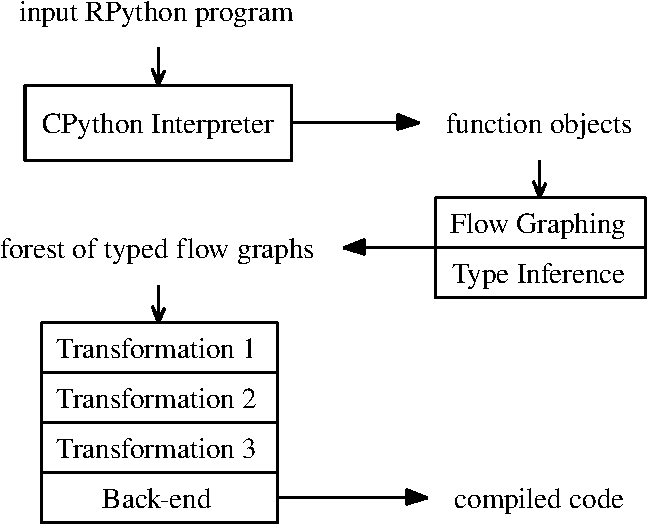
\includegraphics[scale=0.667]{image/arch.pdf}
\caption{overview of the translation process.}
\label{fig_arch}
\end{figure}


\subsection{Transformations}

The first of the transformation steps takes the RPython-typed flow
graphs, still containing polymorphic operations only, and produces
flow graphs with operations more familiar to the target environment.
When the target is C or a C-like environment, this means monomorphic
C-like operations and C-like types.  In the simplest case, this is the
only transformation step: these graphs are directly fed to the C
emitting back-end, which turns them into ANSI C source code.

Not all targets of interest are C-like, though, and we have recently
developed a variant of this step for use when targeting higher-level,
object-oriented (OO) environments.  Its design was motivated by work
on back-ends for Smalltalk/Squeak\footnote{Our simple OO type system
  is designed for \textit{statically-typed} OO environments, including
  Java; the presence of Smalltalk as a back-end might be misleading in
  that respect.} and CLI/.NET.  When targeting a C-like environment,
the first transformation step is called the \textit{LLTyper} or
low-level typer: it produces C-level flow graphs, where the
object-oriented features of RPython (classes and instances) become
manipulations of C structs with explicit virtual table pointers.  By
contrast, for OO environments this step is called the
\textit{OOTyper:} it targets a simple object-oriented type system, and
preserves the classes and instances of the original RPython program.
The LLTyper and OOTyper still have much code in common, to convert the
more Python-specific features like the more complex calling
conventions.  In the sequel, we assume the use of the LLTyper, as
there are as yet no back-ends for the OOTyper which are complete
enough to translate the Standard Interpreter -- although the CLI
backend should be able to within a few months.

For an example of a transformation that is applied after this first
step, consider that RPython has automatic memory management. Even with
the LLTyper, the first transformation step produces flow graphs that
also assume automatic memory management.  Generating C code directly
from there produces a fully leaking program, unless we link it with an
external garbage collector (GC) like the Boehm conservative GC
\cite{Boehm}\cite{boehm-softw}, which is a viable option.

We have two other alternatives, each implemented as a transformation step.
The first one inserts naive reference counting throughout the whole
program's graphs, which without further optimizations gives a somewhat
bad performance (it should be noted that the CPython interpreter is also
based on reference counting, and experience suggests that it was not a
bad choice in this particular case).

The other, and better, alternative is an exact GC, coupled with a
transformation, the \textit{GC transformer}.  It takes as input
C-level-typed graphs and replaces all \texttt{malloc} operations with
calls to a garbage collector's allocation routine.  The transformation
inspects all the graphs to discover the structure types in use
by the program, and assigns a unique type id to each of them.  These
type ids are then collected in internal tables that describe the
layout of the structures, e.g.\ their sizes and the location of the
pointer fields.

We have implemented other transformations as well, e.g.\ performing
various optimizations, or turning the whole code into a style that
allows us to use coroutines (still in ANSI C: it is a variant of
continuation-passing that will be the subject of another paper.)
Another example is the exception transformer, which transforms graphs
that still contain implicit exception handling into a form suitable for
C (currently based on a global flag to signal the presence of an
exception, which is set and checked around selected function calls).

More information about these transformations can be found in \cite{T}.


\subsection{System code}

A common pattern in all the transformation steps is to somehow lower the
level at which the graphs are currently expressed.  Because of this,
there are operations that were atomic in the input (higher-level) graphs
but that need to be decomposed into several operations in the target
(lower-level) graphs.  In some cases, the equivalent functionality
requires more than a couple of operations: a single operation must be
replaced by a call to whole new code -- functions and classes that serve
as helpers.  An example of this is the \texttt{malloc} operation for the GC
transformer.  Another example is the \texttt{list.append()} method, which is
atomic for Python or RPython programs, but needs to be replaced in
C-level code by a helper that possibly reallocates the array of items.

This means that in addition to transforming the existing graphs, each
transformation step also needs to insert new functions into the forest.
A key feature of our approach is that we can write such ``system-level''
code -- relevant only to a particular transformation -- in plain Python
as well.  The idea is to feed these new Python functions into the
front-end, using this time the transformation's target (lower-level)
type system during the type inference.  In other words, we can write
plain Python code that manipulates objects that conform to the
lower-level type system, and turn these functions into graph that are
directly typed in this lower-level type system.

For example, \texttt{ll\textunderscore{}append()} in figure \ref{fig_llappend}
is a Python function
that manipulates objects that behave like C structures and arrays.
This function is inserted by the LLTyper, as a helper to implement the
\texttt{list.append()} calls found in its RPython-level input graphs.
By going through the front-end reconfigured to use C-level types, the
above function becomes a graph with such C-level types,\footnote{The
low-level type system specifies that the function should be
specialized by the C-level type of its input arguments, so it actually
turns into one graph per list type -- list of integers, list of
pointers, etc.  This behavior gives the programmer a feeling
comparable to C++ templates, without the declarations.} which is then
indistinguishable from the other graphs of the forest produced by the
LLTyper.

\begin{figure}
\begin{verbatim}
def ll_append(lst, newitem):
  # Append an item to the end of the vector.
  index = lst.length       #get the 'length' field
  ll_resize(lst, index+1)  #call another helper
  itemsarray = lst.items   #get the 'items' field
  itemsarray[index] = item #behaves like a C array
\end{verbatim}
\caption{a helper to implement \texttt{list.append()}.}
\label{fig_llappend}
\end{figure}

In the example of the \texttt{malloc} operation, replaced by a call to
GC code, this GC code can invoke a complete collection of dead
objects, and can thus be arbitrarily complicated.  Still, our GC code
is entirely written in plain Python, and it manipulates ``objects'' that
are still at a lower level: pointer and address objects.  Even with
the restriction of having to use pointer-like and address-like
objects, Python remains more expressive than, say, C to write a GC
(the work on the Jikes RVM's GC \cite{JikesGC} was the inspiration to try to
express GCs in Python; see section \ref{relatedwork}).

In the sequel, we will call \textit{system code} functions written in
Python that are meant to be analysed by the front-end.  For the
purpose of this article we will restrict this definition to helpers
introduced by transformations, as opposed to the original RPython
program, although the difference is not fundamental to the translation
process (and although our input RPython program, as seen in section
\ref{architecture}, is often itself a Python virtual machine!).

Note that such system code cannot typically be expressed as normal
RPython functions, because it corresponds to primitive operations at
that level.  As an aside, let us remark that the number of primitive
operations at RPython level is, comparatively speaking, quite large:
all list and dictionary operations, instance and class attribute
accesses, many string processing methods, a good subset of all Python
built-in functions...  Compared with other approaches
(e.g.\ Squeak \cite{Squeak}), we
do not try to minimize the number of primitives -- at least not at the
source level.  It is fine to have many primitives at any high enough
level, because they can all be implemented at the next lower level in
a way that makes sense to that level.  The key reason why this is not
burdensome is that the lower level implementations are also written in
Python -- with the only difference that they use (and have to be
typeable in) the lower-level type system.\footnote{This is not strictly
true: the type systems are even allowed to co-exist in the same
function.  The operations involving higher-level type systems are
turned into lower-level operations by the previous transformations in
the chain, which leave the already-low-level operations untouched.}


\subsection{Type systems}

The four levels that we considered so far are summarized in figure
\ref{fig_typesystems}.

\begin{figure}
\centering
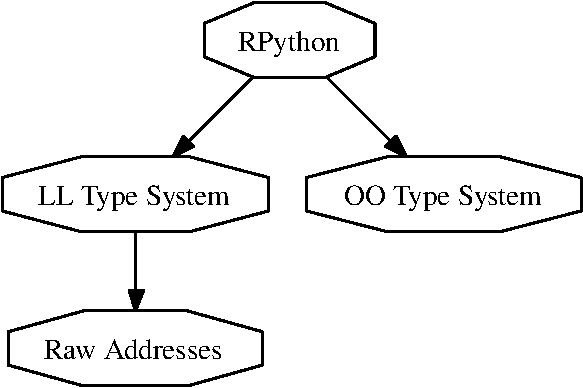
\includegraphics[scale=0.667]{image/typesystems.pdf}
\caption{type systems; the arrows are transformations.}
\label{fig_typesystems}
\end{figure}

The RPython level is a subset of Python, so the types mostly follow
Python types, and the instances of these types are instances in the
normal Python sense; for example where Python has only a single type
\texttt{list}, RPython has a parametric type \texttt{list(T)} for every RPython
type \texttt{T}, but instances of \texttt{list(T)} are just those Python lists
whose items are all instances of \texttt{T}.

The other type systems, however, do not correspond to built-in Python
types.  For each of them, we implemented:
%
\begin{enumerate}
\item The types, which we use to tag the variables of the graphs at
      the given level (types are actually annotated self-recursive
      formal terms, and would have been implemented simply as such if
      Python supported them directly).

\item The Python objects that emulate instances of these types (more
      about them below).
\end{enumerate}
%
We have defined well-typed operations between instances of these types,
syntactically expressed with standard Python operators (e.g.\ if \texttt{x}
is a C-level array, \texttt{x[n]} accesses its \texttt{n}th item).
The emulating instances provide a concrete implementation of
these operations that works in normal Python; the types involved in the
operations are also known to the type inference engine when it
analyses system code like the helper of figure \ref{fig_llappend}.

Now, clearly, the purpose of types like a ``C-like struct'' or a ``C-like
array'' is to be translated to a real \texttt{struct} or array declaration by
the C back-end.  What, then, is the purpose of emulating such things in
Python?  The answer is three-fold.  Firstly, having objects that
live within the Python interpreter, but faithfully emulate the behavior
of their C equivalent while performing additional safety checks, is 
an invaluable help for testing and debugging.  For example, we can
check the correctness of our hash table implementation, written in
Python in term of struct- and array-like objects, just by running it.
The same holds for the GC.

%%% XXX if we're looking to save space, i think this reason can go,
%%% the others seem more important (to me, at least)

Secondly, and anecdotally, as the type inference process (section
\ref{typeinference}) is based on abstract interpretation, we can use
the following trick: the resulting type of most low-level operations
is deduced simply by example.  Sample C-level objects are
instantiated, used as arguments to a given operation, and produce a
sample result, whose C-level type must be the type of the result
variable in the graph.

The third reason is fundamental: we use these emulating objects to
\textit{represent} pre-built objects at that level.  For example, the GC
transformer instantiates an object emulating a C array for the internal
type id table, and fills it with the correct values.  This array
object is then either used directly when testing the GC, or translated
by the C back-end into a static pre-initialized array.

Because our helpers can be both run on top of CPython and translated
we can reuse them both as runtime implementations and to render constant
objects at translation time. This is both natural and useful (especially for complex
data structures). Figure \ref{fig_insertclean} shows a function
implementing insertion in a built-in dictionary for keys known to be
absent, this is used at runtime after resizing and to fill the constant
dictionaries at translation.

\begin{figure}
\begin{verbatim}
def ll_dict_insertclean(d, key, value, hash):
  entry = ll_dict_lookup_clean(d, hash)
  ENTRY = lltype.typeOf(entry).TO
  entry.value = value
  entry.key = key
  if hasattr(ENTRY, 'f_hash'): 
    entry.f_hash = hash
  if hasattr(ENTRY, 'f_valid'):    
    entry.f_valid = True
  if hasattr(ENTRY, 'f_everused'): 
    entry.f_everused = True
  d.num_items += 1
  d.num_pristine_entries -= 1
\end{verbatim}
\caption{built-in dict insertion helper.}
\label{fig_insertclean}
\end{figure}


\section{Type inference}
\label{typeinference}


The various analyses used -- from type inference to lifetime analysis -
are generally formulated as \textit{abstract interpretation.}  While this
approach is known to be less efficient than more tailored algorithms
like constraint-based type inference \cite{Constraint}, we gain in freedom,
controllability and simplicity.  This proved essential in our overall
approach: as described in section \ref{systemprog}, we need to perform
type inference with many different type systems, the details of which
have evolved over time.

We mitigate the potential efficiency problem by wise choices and
compromises for the domain used; the foremost example of this is that
our RPython type inference performs almost no automatic specialization
of functions in the presence of polymorphic arguments.  Another
example is that unlike some schemes which follow exact sets of
concrete run-time classes, we only propagate a single superclass per
variable: the most precise common parent class.  This gives enough
precision for our code generation purposes.  

It is also simple, in the context of abstract interpretation, to
perform translation-time constant propagation, computations and
implement conditional code in a natural way. For example, the code in
figure \ref{fig_insertclean}, which is then specialized for the
possible types of dictionary \texttt{d}, shows this kind of
compile-time computation and introspection on low-level types --
\texttt{ENTRY} is a C-like structure type and the
\texttt{hasattr}-ibute checks introspect it at translation time. This
kind of expressiveness increased our ability to reuse code even in
low-level helpers.

In the sequel, we give a more precise description of this process and
justify our claim that good performance and enough precision can be
achieved -- at least in some contexts -- without giving up the naive but
flexible approach.


\subsection{Building control flow graphs}
\label{flowobjspace}

As described in the overview of the translation process (section
\ref{translationprocess}), the front-end of the translation tool-chain works in
two phases: it first builds control flow graphs from Python functions, and then
performs whole-program type inference on these graphs.

Remember that building the control flow graphs is not done, as one might
first expect, by following a function at the syntactic level.  Instead,
the whole program is imported in a normal Python interpreter -- the full
Python language is used as a kind of preprocessor with
meta-programming capabilities.  Once the program is imported, the object
data in memory consists of Python function objects in bytecode format,
as well as any other kind of objects created at import-time, like class
objects, prebuilt instances of those, prebuilt tables, and so on.  Note
that these objects have typically no text representation any more; for
example, cyclic data structures may have been built at this point.  The
translation tool-chain first turns these function objects into in-memory
control flow graphs which contain direct references to the prebuilt data
objects, and then handles and transforms these graphs.

Figure \ref{fig_screenshot}
shows the control flow graph
obtained for a simple function -- this is a screenshot from our graph
viewer, used for debugging; basic block placement is performed by
Graphviz \cite{graphviz}.

\begin{figure}
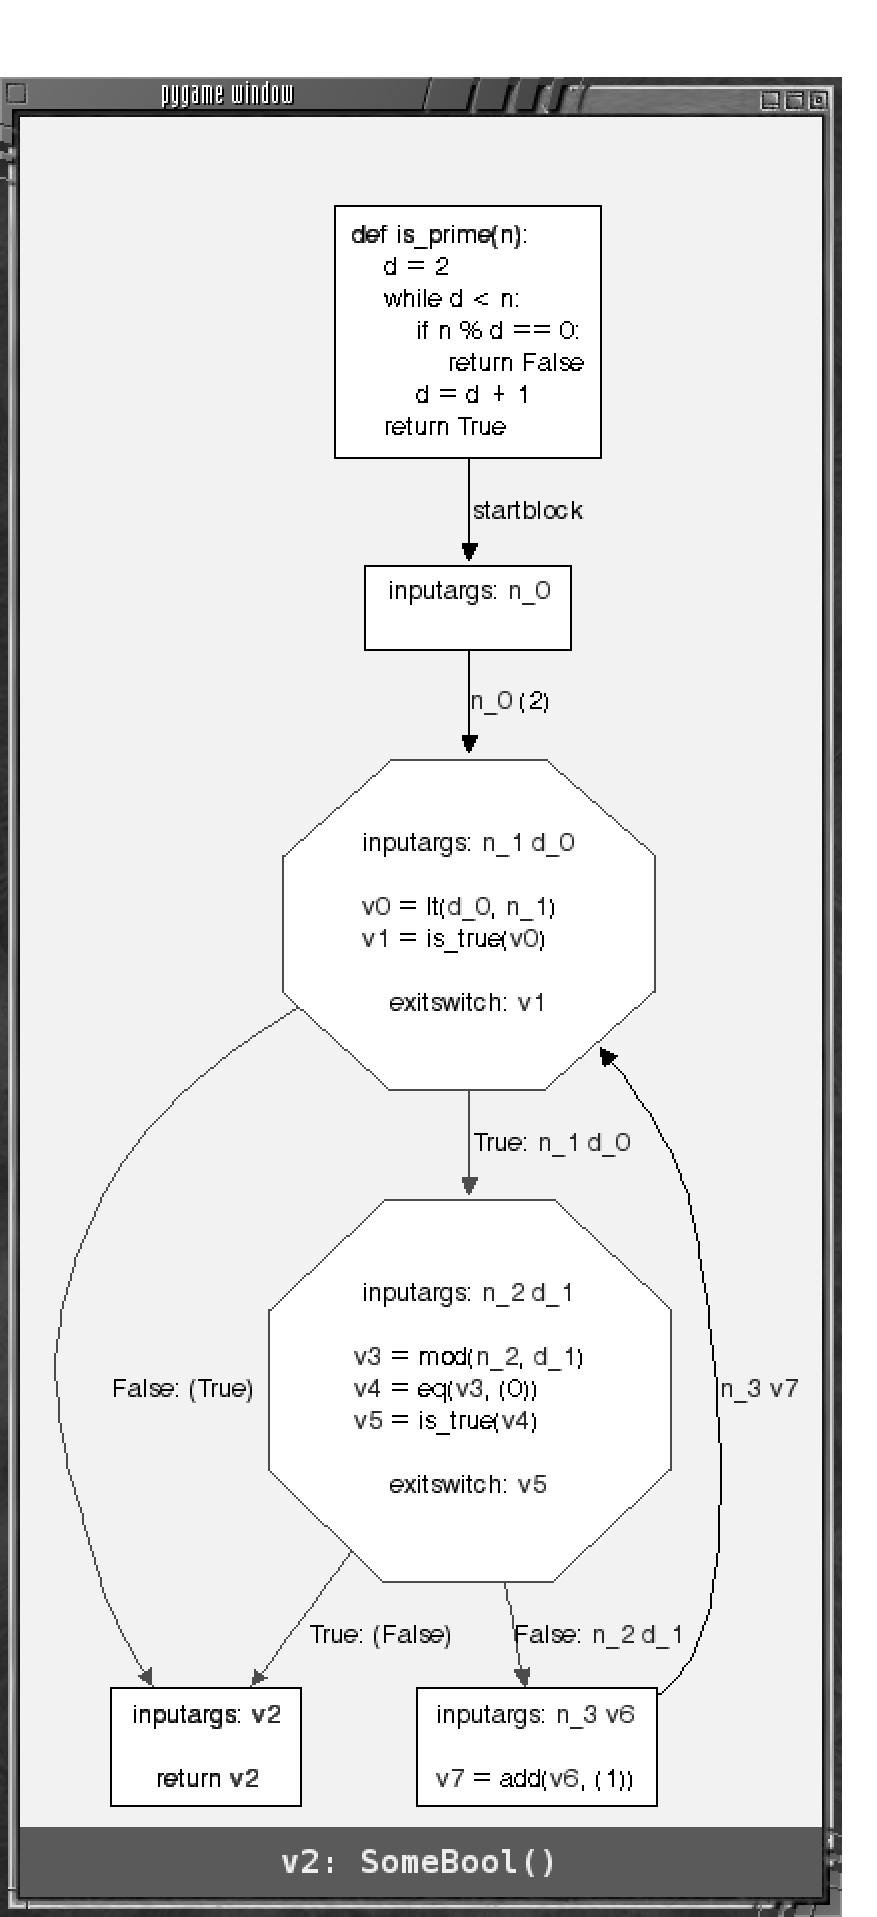
\includegraphics[scale=0.59]{image/screenshot-bw.pdf}
\caption{the control flow graph of a simple function, computed and
displayed by our tool-chain.}
\label{fig_screenshot}
\end{figure}

\begin{figure}
  \centering
  \begin{tabular}{|c|c|} \hline
\multicolumn{2}{|c|}{\vphantom{\Large X}forest of bytecode objects from the application}    \\ \hline
\multicolumn{2}{|c|}{\vphantom{\Large X}Python bytecode interpreter}            \\ \hline
    \vphantom{\Large X} Standard Object Space     &  Flow Object Space  \\ \hline
  \end{tabular}
  \caption{the interpreter and object spaces.}
  \label{fig_interpobjspace}
\end{figure}

The actual transformation from function objects -- i.e.\ bytecode -- to
flow graph is performed by the Flow Object Space, a short but generic
plug-in component for the Python interpreter of PyPy.  The architecture
of our Python interpreter is shown in figure \ref{fig_interpobjspace}.
Note that the left column, i.e.\ the bytecode interpreter and the
Standard Object Space, form the full Python interpreter of PyPy.  It is
an RPython program, and the whole purpose of the translation process is
to accept this as \textit{input}, and translate it to an efficient form.
The description of this particular input program is beyond the scope of
the present paper; see \cite{S}.

However, the bytecode interpreter plays a double role, at two different
levels.  The so-called Object Spaces are \textit{domains} in the abstract
interpretation terminology.  By design, we cleanly separated these
domains from the bytecode interpreter core; the latter is only
responsible for decoding the bytecodes of an application and emulating
the corresponding stack machine.  It treats all actual application-level
objects as black boxes, and dispatches all operations on them to the
Object Space.  The Standard Object Space is a concrete domain, in which
objects are the concrete Python objects of the various built-in types:
lists, dictionaries, and so on.  By opposition, the Flow Object Space is
really an abstract domain.  It handles objects that are placeholders.
Its lattice order (actually a join-semilattice only) is shown in
figure \ref{flowlattice}.

\begin{figure*}
\centering
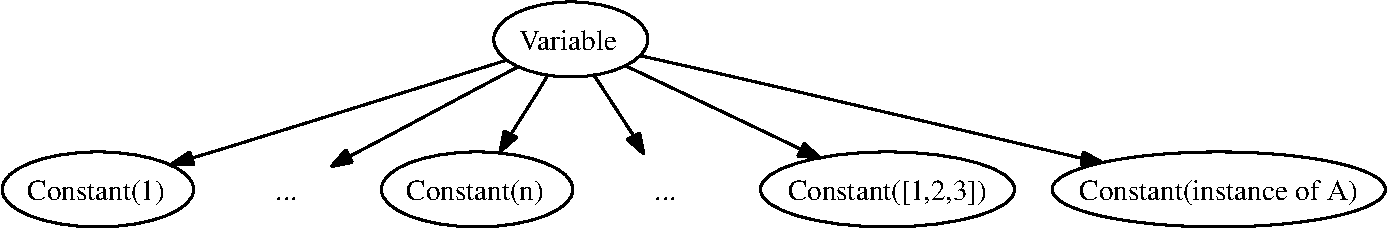
\includegraphics[scale=0.667]{image/flowlattice.pdf}
\caption{the lattice order of the flow object space.}
\label{flowlattice}
\end{figure*}

This order is extremely simple, because most actual analysis is delayed
to the next phase, the type inference engine.  The objects are either
\textit{Variables}, which are pure placeholders for entirely unknown values,
or \textit{Constants} with a concrete Python object as value.  The order places
Variable as the top, and keeps all \textit{Constants} unordered.  Thus if two
different constants merge during abstract interpretation, we immediately
widen them to Variable.

In conjunction with the Flow Object Space, the bytecode interpreter of
PyPy thus performs abstract interpretation of Python bytecodes from
the application.\footnote{Note that this process uses the
\textit{unmodified} bytecode interpreter.  This means that it is
independent of most language details.  Changes in syntax or in
bytecode format or opcode semantics only need to be implemented once,
in the bytecode interpreter.  In effect, the Flow Object Space enables
an interpreter for \textit{any} language to work as a front-end for
the rest of the tool-chain.}  In this case, the bytecodes in
question come from the RPython application that we would like to
translate.

The Flow Object Space records all operations that the bytecode
interpreter ``would like'' to do between the placeholder objects.  It
records them into basic block objects that will eventually be part of
the control flow graph of the whole function.  The recorded operations
take Variables and Constants as argument, and produce new Variables as
results.  The Constants serve two purposes: they are a way to
introduce constant values into the flow graphs -- these values may be
arbitrarily complex objects, not just primitives -- and they allow
basic constant propagation.\footnote{This is useful at this level for
some constructs of the bytecode interpreter, which can temporarily
wrap internal values and push them onto the regular value stack among
the other application-level objects.  We need to be able to unwrap
them again later.  Moreover, we rely on this feature to perform
compile-time computations, particularly in the generic system code
helpers, which ask for and compute with the concrete types of the
variables they receive.}

In the flow graph, branching occurs when the bytecode interpreter tries
to inspect the truth value of placeholder objects, as it would in
response to conditional jump opcodes or other more complicated opcodes:
at this point, the Flow Object Space starts two new basic blocks and -
with a technique akin to continuations -- tricks the interpreter into
following both branches, one after the other.  Additionally, the
bytecode interpreter sends simple positional signals that allow the Flow
Object Space to detect when control paths merge, or when loops close.
In this way, abstract interpretation quickly terminates and the recorded
operations form a graph, which is the control flow graph of the original
bytecode.

Note that we produce flow graphs in Static Single Information or SSI\cite{SSI}
form, an extension of Static Single Assignment\cite{SSA}: each variable is
only used in exactly one basic block.  All variables that are not dead
at the end of a basic block are explicitly carried over to the next
block and renamed, as can be seen in figure \ref{fig_interpobjspace}:
each link carries a list of variables matching the formal input
arguments of its target block.

While the Flow Object Space is quite a short piece of code -- its core
functionality takes only 300 lines -- the detail of the interactions
sketched above is not entirely straightforward; we refer the reader to
\cite{D} for more information.


\subsection{The Annotator}

\begin{figure*}
\centering
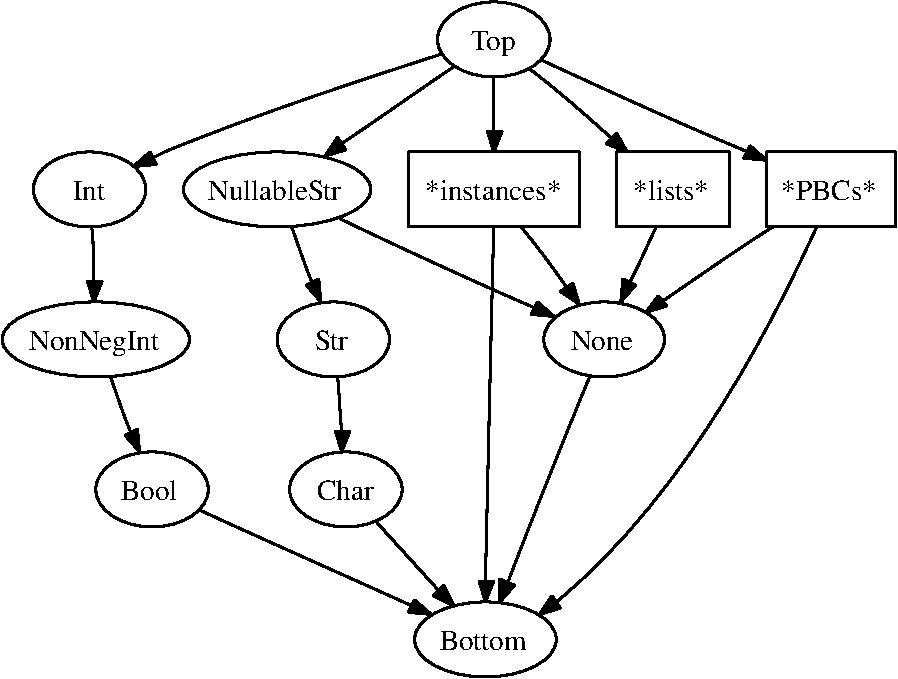
\includegraphics[scale=0.667]{image/lattice1.pdf}
\caption{the overall lattice.}
\label{latticeoverall}
\end{figure*}

The type inference engine, which we call the \textit{annotator}, is the central
component of the front-end part of the translation process.  Given a
program considered as a family of control flow graphs, the annotator
assigns to each variable of each graph a so-called \textit{annotation}, which
describes the possible run-time objects that this variable can contain.
Following usual terminology, we will call such annotations \textit{types} -- not
to be confused with the Python notion of the concrete type of an object.
An annotation is a set of possible values, and such a set is not always
the set of all objects of a specific Python type.

Here is a simplified, static model of how the annotator works.  It can
be considered as taking as input a finite family of functions calling
each other, and working on the control flow graphs of each of these
functions as built by the Flow Object Space (section \ref{flowobjspace}).
Additionally, for a particular ``entry point'' function, the annotator
is provided with user-specified types for the function's arguments.

The goal of the annotator is to find the most precise of our types that can be
given to each variable of all control flow graphs while respecting the
constraints imposed by the operations in which these variables are
involved.

More precisely, it is usually possible to deduce information about the
result variable of an operation given information about its arguments.
For example, we can say that the addition of two integers must be an
integer.  Most programming languages have this property.  However,
Python -- like many languages not specifically designed with type
inference in mind -- does not possess a type system that allows much
useful information to be derived about variables based on how they are
\textit{used}; only on how they were \textit{produced}.  For example,
a number of very different built-in types can be involved in an
addition; the meaning of the addition and the type of the result
depends on the type of the input arguments.  Merely knowing that a
variable will be used in an addition does not give much information
per se.  For this reason, our annotator works by flowing types
forward, operation after operation, i.e.\ by performing abstract
interpretation of the flow graphs.  In a sense, it is a more naive
approach than the one taken by type systems specifically designed to
enable more advanced inference algorithms.  For example,
Hindley-Milner type inference works in an inside-out direction, by
starting from individual operations and propagating type constraints
outwards \cite{DaMi}\cite{Miln}.

Naturally, simply propagating types forward requires the use of a fixed
point algorithm in the presence of loops in the flow graphs or in the
inter-procedural call graph.  Indeed, we flow types forward from the
beginning of the entry point function into each basic block, operation
after operation, and follow all calls recursively.  During this process,
each variable along the way gets a type.  In various cases, e.g.\ when we
close a loop, the previously assigned types can be found to be too
restrictive.  In this case, we generalise them to allow for a larger set
of possible run-time values, and schedule the block where they appear
for reflowing.
The newly generalised types can in turn generalise the types of other
result variables in the block, which in turn can generalise the
types that flow into the following blocks, and so on.  This process
continues until a fixed point is reached.

We can consider that all variables are initially assigned the ``bottom''
type corresponding to the empty set of possible run-time values.  Types
can only ever be generalised, and the model is simple enough to show
that there is no infinite chain of generalization, so that this process
necessarily terminates.


\subsection{RPython types}

As seen in section \ref{systemprog}, we use the annotator with more than one type
systems.  The most interesting and complex one is the RPython type
system, which describes how the input RPython program can be annotated.
The other type systems contain lower-level, C-like types that are mostly
unordered, thus forming more trivial lattices than the one formed by
RPython types.

The set $A$ of RPython types is defined as the following formal terms:
%
\begin{itemize}
\item $Bot$, $Top$ -- the minimum and maximum elements (corresponding
      to ``impossible value'' and ``most general value'');

\item $Int$, $NonNegInt$, $Bool$ -- integers, known-non-negative
      integers, booleans;

\item $Str$, $Char$ -- strings, characters (which are strings of
      length 1);

\item $Inst(class)$ -- instance of $class$ or a subclass thereof
      (there is one such term per $class$);

\item $List(v)$ -- list; $v$ is a variable summarising the items of
      the list (there is one such term per variable);

\item $Pbc(set)$ -- where the $set$ is a subset of the (finite) set of
      all prebuilt constant objects.  This set includes all the
      callables of the input program: functions, classes, and methods.

\item $None$ -- stands for the singleton \texttt{None} object of
      Python.

\item $NullableStr$, $NullableInst(class)$ -- a string or
      \texttt{None}; resp. an instance or \texttt{None}.
\end{itemize}

Figures \ref{latticeoverall} and \ref{latticedetail} show how these
types are ordered to form a lattice -- we generally use its structure of
join-semilattice only, but we will see in section \ref{precision}
a use case for the \textit{meet}.
Not shown on the figures are the list terms, which are simply
unordered with each other, and the Pbcs, which form a
classical finite set-of-subsets lattice.  In addition, we have left
out a number of other annotations that are irrelevant for the basic
description of the annotator and straightforward to handle:
$Dictionary$, $Tuple$, $Float$, $UnicodePoint$, $Iterator$, etc.  The
complete list is described in \cite{T}.

\begin{figure}
\centering
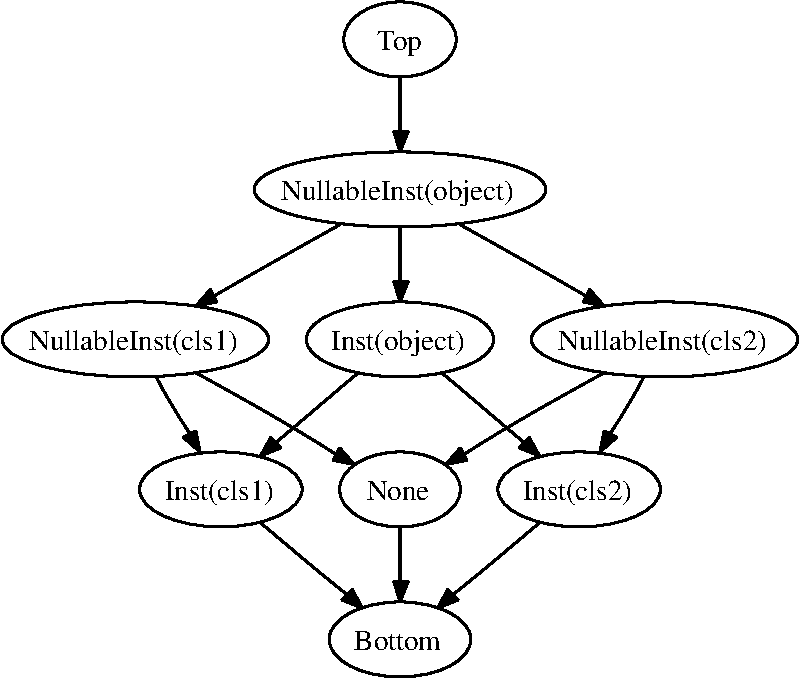
\includegraphics[scale=0.667]{image/lattice2.pdf}
\caption{the part about instances and nullable instances, assuming a
  simple class hierarchy with only two direct subclasses of
  \texttt{object}.}
\label{latticedetail}
\end{figure}

The type system moreover comes with a family of rules, which for every
operation and every meaningful combination of input types describes the
type of its result variable.  Let $V$ be the set of Variables that
appear in the user program's flow graphs.  Let $b$ be a map from $V$
to $A$; it is a ``binding'' that gives to each variable a type.  The
purpose of the annotator is to compute such a binding stepwise.

Let $x$, $y$ and $z$ be Variables.  We introduce the rules:
%
$$
\begin{array}{c}
 z = \mathrm{add}(x, y), \; b(x) =
    Int, \; b(y) = Int \\ \hline
 b' = b \hbox{\ with\ } (z
    \rightarrow Int) 
\end{array}
$$
%
$$
\begin{array}{c}
 z = \mathrm{add}(x, y), \; Bool \leq b(x), b(y) \leq
    NonNegInt \\ \hline
 b' = b \hbox{\ with\ } (z
    \rightarrow NonNegInt) 
\end{array}
$$
%
The first rule specifies that if we see the addition operation applied to
Variables whose current binding is $Int$, a new binding $b'$ can be
produced: it is $b$ except on $z$, where we have $b'(z) = Int$.
The second rule specifies that in a similar case, if both arguments are
known to be non-negative, so is the result.  Extra rules control addition
between other combinations of numbers, as well as strings, lists and tuples
(for which addition is concatenation).  Similar sets of rules are
introduced for each operation.

The type inference engine can be seen as applying this kind of rules
repeatedly.  It does not apply them in random order, but follows a
forward-propagation order typical of abstract interpretation.

It is outside the scope of the present paper to describe the type
inference engine and the rules more formally.  The difficult points
involve mutable containers, e.g.\ initially empty list that are
filled somewhere else; the discovery of instance attributes --
in Python, classes do not declare upfront a fixed set of attributes
for their instances, let alone their types; and the discovery of
base class interfaces -- across a class hierarchy, some methods with
the same name may be called polymorphically by the program, while
others may be unrelated methods used internally by the subclasses.
These examples require reflowing techniques that invalidate existing
types in already-annotated basic blocks, to account for the influence
of more general types coming indirectly from a possibly distant part
of the program.  The reader is referred to \cite{D}
for more information.


\subsection{Termination and complexity}

The lattice model clearly contains no infinite chain.  Moreover, it is
designed to convince oneself that the number of reflowings required in
practice is small.  For example, we are not trying to do range analysis
beyond detecting non-negatives -- the reason is that range analysis is
not an essential part of writing \textit{reasonably} efficient code.  Consider
that a translated RPython program runs hundreds of times faster than
when the same program is executed by the standard Python interpreter: in
this context, range analysis appears less critical.  It is a possible
optimization that we can introduce in a later, optional analysis and
transformation step.

The worst case behaviors that can appear in the model described above
involve the lattice of Pbcs, involving variables that could contain
e.g.\ one function object among many.  An example of such behavior is
code manipulating a table of function objects: when an item is read
out of the table, its type is a large Pbc set: $Pbc(\{f_1, f_2, f_3,
\ldots\})$.  But in this example, the whole set is available at once,
and not built incrementally by successive discoveries.  This seems to
be often the case in practice: it is not very common for programs to
manipulate objects that belong to a large but finite family -- and when
they do, the whole family tends to be available early on, requiring
few reflowings.

This means that \textit{in practice} the complete process requires a time that
is far lower than the worst case.  We have experimentally confirmed
this: annotating the whole PyPy interpreter (90,000 lines) takes on the
order of 5 to 10 minutes, and basic blocks are typically only reflown a
handful of times, providing a close-to-linear practical complexity.

We give formal termination and correctness proofs in \cite{D}, as well as
worst-case bounds and common-case estimates.


\subsection{Precision}
\label{precision}

Of course, this would be pointless if the annotation did not give
precise enough information for our needs.  We must describe a detail of
the abstract interpretation engine that is critical for precision: the
propagation of conditional types.  Consider the following source code
fragment:
%
\begin{verbatim}
    if isinstance(x, MyClass):
        f(x)
    else:
        g(x)
\end{verbatim}
%
Although the type of \texttt{x} may be some parent class of
\texttt{MyClass}, within the positive branch of the \texttt{if} it can
be deduced to be of the more precise type $Inst(MyClass)$.\footnote{Remember
 that our graphs are in SSI form, which means
that the \texttt{x} inside each basic block is a different Variable
with a possibly different type as annotation.  Given that our type
inference is not flow-sensitive, SSI gives an advantage over SSA
here.}

This is implemented by introducing an extended family of types for
boolean values:
%
$$
Bool(v_1: (t_1, f_1), v_2: (t_2, f_2), ...)
$$
%
where the $v_n$ are variables and $t_n$ and $f_n$ are types.  The
result of a check, like \texttt{isintance()} above, is typically
annotated with such an extended $Bool$.  The meaning of the type is as
follows: if the run-time value of the boolean is True, then we know
that each variable $v_n$ has a type at most as general as $t_n$; and
if the boolean is False, then each variable $v_n$ has a type at most
as general as $f_n$.  This information is propagated from the check
operation to the exit of the block via such an extended $Bool$ type,
and the conditional exit logic in the type inference engine uses it to
trim the types it propagates into the next blocks (this is where the
\textit{meet} of the lattice is used).

With the help of the above technique, we achieve a reasonable precision
in small examples.  For larger examples, a different, non-local
technique is required: the specialization of type-polymorphic functions.

As described in the introduction, the most important downside of our
approach is that automatic specialization is a potential
performance-killer.  So we decided that in the normal case, all calls to
a given function contribute to a single annotation of that function.
Inside the function graph, we propagate the \textit{join} of the types
of the actual parameters of the call sites.  We \textit{do} support
specialization, however: we can generate several independently-annotated
copies of the flow graph of certain functions.  When annotating RPython
programs, such specialization does not happen automatically: we rely on
hints provided by the programmer in the source code, in the form of
flags attached to function objects.  As we had this trade-off in mind
when we wrote the Python interpreter of PyPy, we only had to add about
a dozen hints in the end.

This does not mean that automatic specialization policies are difficult
to implement.  Indeed, the simpler lower-level type systems rely quite
heavily on them: this is because the system code helpers are often
generic and can receive arguments of various C-level types.  In this
case, because the types at this level are limited and mostly unordered,
specializing all functions on their input argument's types works well.

At the level of RPython, the range of specializations
that make sense is actually much wider.  Although we only specialize a
very small subset of the functions, we use criteria as diverse as
specialization by the type of an argument, specialization by an
expected-to-be-constant argument value, memoized functions that the
type inference engine will actually call during annotation and replace
by look-up tables, and even complete overriding of the annotator's behavior in
extreme cases.  In this sense, the need for manual specialization turned
into an advantage, in term of simplicity and flexibility of implementing
and using new specialization schemes.

This conclusion can be generalised.  We experimented with a simple
approach to type inference that works well in practice, and that can
very flexibly accomodate small and big changes in the type system.
We think that the reasons for this success are
to be found on the one hand in the (reasonable) restrictions we put on
ourselves when designing the RPython language and writing the Python
interpreter of PyPy in RPython, and on the other hand in an ad-hoc type
system that is designed to produce enough precision (but not more) for
the purpose of the subsequent transformations to C-level code.

We should mention that restricting oneself to write RPython code instead
of Python is still a burden, and that we are not proposing in any way
that the Python language itself should evolve in this direction, nor
even that RPython usage should become widespread.  It is a tool designed
with a specific goal in mind, which is the ability to produce reasonably
efficient, stand-alone code in a large variety of environment.



\section{Experimental results}
\label{experimentalresults}


\subsection{Performance}

Our tool-chain is capable of translating the Python interpreter of
PyPy, written in RPython, currently producing either ANSI C code as
described before, or LLVM\footnote{
The LLVM \cite{LLVM:CGO04} project is the realization
of a portable assembler infrastructure, offering both a virtual
machine with JIT capabilities and static compilation. Currently we are
using the latter with its good high-level optimizations for PyPy.}
assembler which is then compiled to native code with LLVM tools.

The tool-chain has been tested with and can sucessfully apply
transformations enabling various combinations of features. The
translated interpreters are benchmarked using pystone (a Dhrystone 2.0
\cite{dhry20} derivative traditionally used by the Python community,
although it is a rather poor benchmark) and the classical Richards
benchmark (ported to Python) and compared against CPython 2.4.3 \cite{cpy243}.
Results are summarized in table \ref{perfsumm}.

\begin{table*}
% the layout of this table isn't wonderful, but it's probably OK.
\centering
\begin{tabular}{|l|c|c|} \hline
\textbf{Interpreter} & 
\textbf{Richards, Time/iteration} &
\textbf{Pystone, Iterations/second} \\ \hline
CPython 2.4.3                &   789ms  (1.0x) & 40322  (1.0x) \\ \hline
pypy-c                       &  4269ms  (5.4x) &  7587  (5.3x) \\ \hline
pypy-c-thread                &  4552ms  (5.8x) &  7122  (5.7x) \\ \hline
pypy-c-stackless             &  5121ms  (6.5x) &  6060  (6.7x) \\ \hline
pypy-c-gcframework           &  6327ms  (8.0x) &  4960  (8.1x) \\ \hline
pypy-c-stackless-gcframework &  8743ms (11.0x) &  3755 (10.7x) \\ \hline
pypy-llvm-c                  &  3797ms  (4.8x) &  7763  (5.2x) \\ \hline
pypy-llvm-c-prof             &  2772ms  (3.5x) & 10245  (3.9x) \\ \hline
\end{tabular}
\caption{summary of interpreter performance.}
\label{perfsumm}
\end{table*}

The numbers in parenthesis are slow-down factors compared to CPython.
These measures reflect PyPy revision 27815\footnote{PyPy is an open-source project
under the MIT license, PyPy source repository using subversion lives at 
http://codespeak.net/svn/pypy/dist/.}, 
compiled with GCC 3.4.4.  LLVM is version 1.8cvs (May 11, 2006).  The
machine runs GNU/Linux SMP on an Intel(R) Pentium(R) 4 CPU at 3.20GHz
with 2GB of RAM and 1MB of cache.  The rows correspond to variants of
the translation process, as follows:

{\bf pypy-c:}
    the simplest variant; translated to C code with no explicit memory
    management, and linked with the Boehm conservative GC.

{\bf pypy-c-thread:}
    the same, with OS thread support enabled (thread support is kept
    separate for measurement purposes because it has an impact on the
    GC performance).

{\bf pypy-c-stackless:}
    the same as pypy-c, plus the ``stackless transformation'' step which
    modifies the flow graph of all functions to allow them
    to save and restore their local state, as a way to enable coroutines.

{\bf pypy-c-gcframework:}
    in this variant, the ``gc transformation'' step inserts explicit
    memory management and a simple mark-and-sweep GC implementation.
    The resulting program is not linked with Boehm.  Note that it is not
    possible to find all roots from the C stack in portable C; instead,
    in this variant each function explicitly pushes and pops all roots
    to an alternate stack around each subcall.

{\bf pypy-c-stackless-gcframework:}
    this variant combines the ``gc transformation'' step with the
    ``stackless transformation'' step.  The overhead introduced by the
    stackless feature is theoretically balanced with the removal of the
    overhead of pushing and popping roots explicitly on an alternate
    stack: indeed, in this variant it is possible to ask the functions
    in the current C call chain to save their local state and return.
    This has the side-effect of moving all roots to the heap, where the
    GC can find them.  (We hypothesize that the large slowdown is caused
    by the extreme size of the executable in this case -- 21MB, compared to
    6MB for the basic pypy-c.  Making it smaller is work in progress.)

{\bf pypy-llvm-c:}
    the same as pypy-c, but using the LLVM back-end instead of the C
    back-end.  The LLVM assembler-compiler gives the best results when -
    as we do here -- it optimizes its input and generates again C code,
    which is fed to GCC.

{\bf pypy-llvm-c-prof:}
    the same as pypy-llvm-c, but using GCC's profile-driven
    optimizations.

The speed difference with CPython 2.4.3 can be explained at two levels.
One is that CPython is hand-crafted C code that has been continuously
optimized for a decade now, whereas the Python interpreter of PyPy first
seeks flexibility and high abstraction levels.  The other, probably
dominant, factor is that various indices show that our approach places a
very high load on the GC and on the memory caches of the machine.  The
Boehm GC is known to be less efficient than a more customized approach;
kernel-level profiling shows that pypy-c typically spends 30\% of its
time in the Boehm library.  Our current, naively simple mark-and-sweep
GC manages to be a bit worse.  The interaction with processor caches is
also hard to predict and account for; in general, we tend to produce
quite large amounts of code and prebuilt data.  The overall performance
is still reasonable: some variants are within the same order of
magnitude as CPython, while others trade a slow-down for functionalities
not available in CPython.


\subsection{Translation times}

A complete translation of the pypy-c variant takes about 39 minutes,
divided as shown in table \ref{translationtimes}.

\begin{table*}
\centering
\begin{tabular}{|p{0.65\linewidth}|c|} \hline
\textbf{Step} & \textbf{Time (minutes:seconds)} \\ \hline
Front-end                                 
(flow graphs and type inference)          
& 9:01 \\ \hline
LLTyper                                   
(from RPython-level to C-level graphs     
and data)                                 
& 10:38 \\ \hline
Various low-level optimizations           
(convert some heap allocations to local   
variables, inlining, ...)                 
& 6:51 \\ \hline
Database building                         
(this initial back-end step follows all   
graphs and prebuilt data structures       
recursively, assigns names, and orders    
them suitably for code generation)        
& 8:39 \\ \hline
Generating C source                       
& 2:25 \\ \hline
Compiling (\texttt{gcc -O2})              
& 3:23 \\ \hline
\end{tabular}
\caption{dividing overall translation time by stage.}
\label{translationtimes}
\end{table*}

An interesting feature of this table is that type inference is not the
bottleneck.  Indeed, further transformation steps typically take longer
than type inference alone.  This is the case for the LLTyper step,
although it has a linear complexity on the size of its input (most
transformations do).

Other transformations like the ``gc'' and the ``stackless'' ones actually
take more time, particuarly when used in combination with each other (we
speculate it is because of the increase in size caused by the previous
transformations).  A translation of pypy-c-stackless, without counting
GCC time, takes 60 minutes; the same for pypy-c-stackless-gcframework
takes 129 minutes.



\section{Future work}
\label{futurework}


As described in section \ref{experimentalresults}, the performance of
the compiled Python interpreters is not yet up to competing with the
well-established CPython.  We are always working to improve matters,
considering new optimizations and better GCs.

Current work also includes refininments of the OOTyper and work on
back-ends that use it, including those targeting CLI/.NET and
Smalltalk/Squeak.


\subsection{JIT Specializer}

So far, the PyPy tool-chain can only translate the Python interpreter of
PyPy into a program which is again an interpreter -- the same interpreter
translated to C, essentially, although we have already shown that some
aspects can be ``weaved'' in at translation time, like support for
coroutines.

To achieve high performance for dynamic languages such as Python, the
proven approach is to use dynamic compilation techniques, i.e.\ to write
JITs.  With direct techniques, this is a major endeavour, and
increases the effort involved in further evolution of the language.

In the context of the PyPy project, we are now exploring -- as we planned
from the start -- the possibility of producing a JIT as a graph
transformation aspect from the Python interpreter.  This idea is based
on the theoretical possibiliy to turn interpreters into compilers by
partial evaluation\cite{Jones:1993:PartialEvaluation}.
In our approach, this is done by analysing
the forest of flow graphs built from the Python interpreter, which is a
well-suited input for this kind of techniques.  We can currently perform
binding-time analysis on these graphs, again with abstract
interpretation techniques reusing the type inference engine.  The next
step is to transform the graphs -- following the binding-time annotations
-- into a compiler; more precisely, in partial evalution terminology, a
generating extension.  We can currently do this on trivial examples.

The resulting generating extension will be essentially similar to
Psyco \cite{psyco}, which is the only (and hand-written) JIT available for Python
so far, based on run-time specialization.



\section{Related work}
\label{relatedwork}


Applying the expressiveness -- or at least the syntax -- of very
high-level and dynamically typed languages to their implementation has
been investigated many times.

One typical approach is writing a static compiler.  The viability of,
and effort required for, such an approach depends usually on the binding
and dispatch semantics of the language.  Common Lisp native compilers,
usable interactively and taking single functions or files as compilation
units, are a well-known example of that approach.  However, the late
binding for all names and the load semantics make such an approach very
hard for Python, if speed improvements are desired.

In this context, it is more relevant to consider and compare with
projects using dynamic and very-high-level languages for interpreters
and VM implementations, and Just-In-Time compilers.

Scheme48 was a Scheme implementation using a restricted Scheme, PreScheme
\cite{kelsey-prescheme}, with static type inference based on Hindley-Milner.  This is
viable for Scheme as base language.  Simplicity and portability across C
platforms were its major goals.

Squeak \cite{Squeak} is a Smalltalk implementation in Smalltalk. It uses SLang, a
very restricted subset of Smalltalk with few types and strict
conventions, which can be mostly directly translated to C.
The VM, the object memory and the garbage collector support are
explicitly written together in this style. Again simplicity and
portability were the major goals, as opposed to sophisticated manipulation
and analysis or ``weaving'' in of features as transformation aspects.

Jikes RVM \cite{jalapeno} is a
Java VM and Just-In-Time compiler written in Java.
Bootstrapping happens by self-applying the compiler on a host VM, and
dumping a snapshot from memory of the resulting native code.
This approach directly enables high performance, at the price of
portability -- as usual with pure native code emitting
approaches. Modularity of features, when possible, is achieved with
normal software modularity. The indirection costs are taken care of by
the compiler performing inlining (which is sometimes even explicitly
requested).  In particular this modular approach is used
for implementing a range of choices for GC support \cite{JikesGC}.  This was
the inspiration for PyPy's own GC framework, although much more tuning
and work went into Jikes RVM.  PyPy's own GC framework also exploits
inlining of helpers and barriers to recover performance.

Jikes RVM's native JIT compilers \cite{Jikes-JIT}
are not meant to be retargetted to run in other environments
than hardware processors, for example in a CLR/.NET
runtime. Also Jikes RVM pays the complexity of writing
a JIT up-front, which also means that features and semantics of the
language are encoded in the JIT compiler code.  Major changes of the
language are likely to correspond to major surgery of the JIT.

PyPy's more indirect approach, together hopefully with our future work
on generating a JIT compiler, tries to overcome these limitations, at
the price of some more efforts required to achieve very good
performance. It is too soon for a complete comparison of the complexity,
performance and trade-offs of these approaches.



\section{Conclusion}
\label{conclusion}


The PyPy project aims at showing that dynamic languages are suitable and
quite useful for writing virtual machines in.  We believe that we have
achieved this objective.  The present paper gave an overview of the
architecture that enabled this result.  Experiments suggest that
practical virtual machines could reasonably follow in the near future,
with faster-than-current virtual machines with JIT specialization
techniques for the mid-term future.

Targetting platforms that are very different from C/Posix is work in
progress, but given that many of the initial components are shared with
the existing stack of transformations leading to C, we are confident
that this work will soon give results.  Moreover, we believe that these
results will show reasonable efficiency, because our back-ends for VMs
like Squeak and .NET can take advantage of a high-level input (as opposed
to trying to translate, say, C-like code to Smalltalk).

A desirable property of our approach is to allow a given language and VM
to be specified only once, in the form of an interpreter.  Moreover, the
interpreter can be kept simple (and thus keep its role as a
specification): not only is it written in a high-level language, but it
is not overloaded with low-level design choices and implementation
details.  This makes language evolution and experimentation easier.
More generally, this property is important because many interpreters for
very difference languages can be written: the simpler these interpreters
can be kept, the more we win from our investment in writing the
tool-chain itself -- a one-time effort.

Dynamic languages enable the definition of multiple custom type systems,
similar to \textit{pluggable type systems} in \cite{PlugType} but with simple
type inference instead of explicit annotations.  This proved a key
feature in implementing our translation tool-chain, because it makes a
many-levels approach convenient: each abstraction level can provide an
implementation for some of the features that the higher levels
considered primitive.  It offsets the need to define a minimal kernel of
primitives and build everything on top of it; instead, we have been able
to implement, so to speak, the right feature at the right level.

\bigskip

\bibliographystyle{abbrv}
\bibliography{paper}

\end{document}
